\usetikzlibrary{calc}
\usetikzlibrary{chains, decorations.pathreplacing, positioning}

\definecolor{decoration}{RGB}{0, 122, 195} %CTU blue
\definecolor{heading}{RGB}{0, 122, 195}
\definecolor{headbackgroundgray}{RGB}{199, 219, 241} %light blue
\definecolor{backgroundgray}{RGB}{199, 219, 241} %CTU light blue
\definecolor{headgray}{rgb}{0.50,0.50,0.51}
\definecolor{enumgray}{RGB}{0, 122, 195} %CTU blue

\begin{figure}[ht]
\centering
\caption{The two-dimensional finite difference grid}
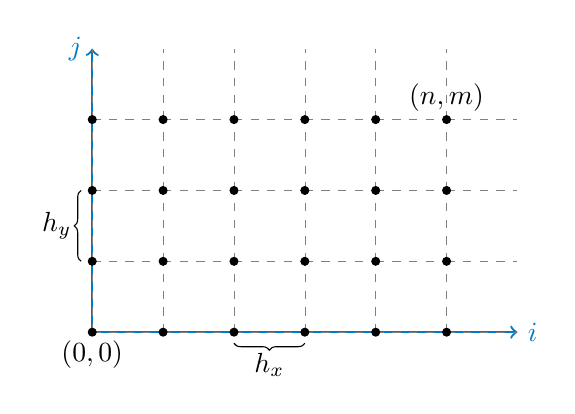
\begin{tikzpicture}[scale=0.9]

\tikzstyle{annot} = [text width=4em, text centered]

\draw [->, thick,enumgray] (0,0) -- (0,4) node[anchor=east] {$j$};
\draw [->, thick,enumgray] (0,0) -- (6,0) node[anchor=west] {$i$};

\draw [decorate, decoration = {brace, raise = 4pt}] (0,1) -- (0,2) node[pos=0.5,left=4pt,black] {$h_y$};
\draw [decorate, decoration = {mirror, brace, raise = 4pt}] (2,0) -- (3,0) node[pos=0.5,below=4pt,black] {$h_x$};

\foreach \x in {0, ..., 5}{
  \foreach \y in {0, ..., 3} {
    \draw [style=help lines,dashed] (\x,\y) -- (\x+1,\y);
    \draw [style=help lines,dashed] (\x,\y) -- (\x,\y+1);

    \node[draw,circle,inner sep=1pt,fill] (vertex\x\y) at (\x,\y) {};
  }
}

\node[annot, below of=vertex00, node distance=8pt] {$(0,0)$};
\node[annot, above of=vertex53, node distance=8pt] {$(n,m)$};

\end{tikzpicture}

\label{FDM-2D-grid}
\end{figure}